\documentclass[12pt]{report}

\usepackage{indentfirst}
\usepackage{hyperref}
\usepackage{graphicx}
\usepackage[margin=1in]{geometry}

\graphicspath{ {../data/003/visualisation_v2/} {../results/SLP/003/ROC/} }

\setcounter{secnumdepth}{0}

\begin{document}
	\begin{center}
	    \vspace*{1cm}
	    \Large
	    VILNIUS UNIVERSITY
	    
	    \vspace*{4cm}
        \Large
        IEVA PUDŽIUVELYTĖ
	    
        \vspace*{2cm}
        \Large
        PROTEIN THERMOSTABILITY PREDICTION USING 
		SEQUENCE REPRESENTATIONS FROM PROTEIN 
		LANGUAGE MODELS 
        
        \vspace*{2cm}
        \large
        Course thesis
        
        \vspace*{2cm}
        \large
        Vilnius, 2022
        
	\end{center}
	
	\newpage

	\tableofcontents

	\newpage
	
	\Large
	\section{Introduction}

    \vspace*{1cm}
        
	\normalsize

	The variety of proteins is no less diverse than the variety of organisms. 
	Just as the latter set is divided into domains, there are different 
	attempts to classify proteins into distinct subsets. One way is to 
	consider the heat-resistance property of biological macromolecules, which 
	is an important trait for practical applications, for example, PCR.

	Earlier studies show that protein's sequence and structural properties 
	influence the thermostability of the macromolecule (Modarres et al. 2016). 
	Furthermore, one of the most recent achievements in the field of deep 
	learning are transformer architecture-based language models or, particularly, 
	protein language models that have not yet been used to classify proteins based on
	their thermostability. Therefore, it was decided to apply protein 
	representations from the protein language model to make inferences about 
	thermostability of the biological macromolecules.

	There are transformer architecture-based language models trained in an 
	unsupervised fashion to predict probabilities of elements in sequences 
	(Devlin et al. 2018). 
	Simultaneously, the process of training creates sequences' embeddings – the 
	real numbered vectors that represent semantic connections of language 
	components. These representations can be transferred as input to specific 
	application models trained using a supervised learning method to complete 
	the defined task, such as the classification problem. Unsurprisingly, the 
	transition between two types of learning has a name of 'transfer learning'. 
	This separation is practically useful because the computationally-heavy 
	task to train the language model can be excluded from the development of 
	the application model.

	Since proteins can be represented in amino acid sequences assumed as a 
	particular language, there are protein language models – models trained on 
	protein sequences – that provide embeddings as output. The multi-dimensional 
	vectors are transferred for the application neural network as its input to 
	observe the results and decide whether the computed representations are 
	suitable to solve the specific biological task.

	This work presents a novel way to predict thermal stability of proteins. 
	The solution is a feed-forward neural network (FNN). To train the FNN, 
	the evolutionary scale model 1b (ESM-1b) (Rives et al. 2021) is used to 
	generate embeddings for proteins of organisms with annotated growth 
	temperatures (Engqvist 2018). The model 
	takes the generated embedding to predict the thermostability class of the 
	input protein.

	\newpage

	\section{Theory}

	The main objective of the work is to create a classifier that could 
	determine to which thermostability class the protein sequence belongs.

	Thermostability classes were created by setting the threshold of 
	$65\ ^\circ$C - proteins that are stable at temperatures strictly lower 
	than the given threshold should be assigned to class '0' and the 
	remaining ones compose the class '1'. 

	\subsection{ESM-1b embeddings}

	Due to the novelty of embeddings, a considerably good performance of
	protein language models, and a recently emerged availability of embeddings,
	it was decided to develop a neural network model that would take protein
	embeddings from ESM-1b model as input and give the thermostability class
	label as output.

	ESM-1b is one of evolutionary scale models trained by Facebook Research 
	(Rives et al. 2021). The model has 33 layers and 650 million parameters. 
	The model was trained in an 
	unsupervised fashion on UniRef50 dataset (accessed March 28, 2018). In order to ensure
	determinism in the validation set, authors removed protein sequences that
	were longer than 1024 amino acids. 

	The authors made a script to extract model's embeddings available in the 
	repository "Evolutionary Scale Modeling". The script allows to choose 
	from which model and layer embeddings will be taken, what embeddings 
	(mean, per amino acid, or beginning of the sequence token) to keep. In the
	result of using the script, a 1280 dimensional vector for each protein is 
	generated.
	
	The fact that sequences longer than 1024 amino acids were removed from the 
	validation dataset for ESM-1b model's training implies to the limitation of 
	model's embeddings, which cannot be generated for sequences longer than 
	1024 amino acids. For this reason, various methods to get the most accurate 
	prediction for longer sequences were tried.

	\newpage

	\section{Methods}

	Generally, the workflow consisted of the following steps:

	\begin{enumerate}
		\item Collecting sets of sequences
		\item Calculating ESM-1b embeddings for the sets of sequences
		\item Processing the set of generated embeddings
		\item Visualising ESM-1b embeddings
		\item Training and validating the neural network model of the chosen architecture 
		\item Testing the trained neural network model
		\item Presenting the results of the model
	\end{enumerate}

	The workflow will be reviewed in terms of these points.

	\subsection{Collecting data}

	Initially, the steps prior to the neural network model construction 
	were done using a small dataset that was composed of proteomes of two 
	organisms: a mesophilic bacteria \textit{Escherichia coli} 
	(\href{https://www.uniprot.org/proteomes/UP000000625}{UP000000625}) and a 
	thermophilic archaeon \textit{Sulfolobus solfataricus} 
	(\href{https://www.uniprot.org/proteomes/UP000001974}{UP000001974}). The 
	growth temperature of \textit{E. coli} is $37\ ^\circ$C (Jang et al. 2017) 
	and $80\ ^\circ$C for \textit{S. solfataricus} (Zaparty et al. 2010). This 
	dataset was named '001' and used only for embeddings visualisation.

	The visualisation of '001' stimulated to check whether embeddings are 
	distinguished by the thermostability property or the life domain has a
	significant impact to the data clusterisation. Subsequently, '002' dataset 
	was a collection of 2 mesophilic archaea and 2 thermophilic bacteria
	proteomes.

	\vspace*{0.5cm}

	Mesophilic archaea:

	\begin{itemize}
		\item \textit{Methanobrevibacter oralis} 
		(\href{https://www.uniprot.org/proteomes/UP000077428}{UP000077428})
		\item \textit{Nitrosopumilus maritimus} strain SCM1 (\href{https://www.uniprot.org/proteomes/UP000000792}{UP000000792})
	\end{itemize}

	Thermophilic bacteria:

	\begin{itemize}
		\item \textit{Aquifex aeolicus} (strain VF5)
		(\href{https://www.uniprot.org/proteomes/UP000000798}{UP000000798})
		\item \textit{Thermotoga maritima} 
		(strain ATCC 43589 / DSM 3109 / JCM 10099 / NBRC 100826 / MSB8) 
		(\href{https://www.uniprot.org/proteomes/UP000008183}{UP000008183})
	\end{itemize}

	After receiving the results of the first neural network model, it was decided
	to train and test the model on the first real dataset. '003' dataset was a subset
	of the dataset of 21458 annotated organisms (Engqvist 2018). 
	
	Requirements for '003' dataset were: the dataset needed to be balanced and a
	single taxonomy identifier could be apparent only in either training, validation,
	or testing dataset. 
	
	To make the dataset balanced, 216595 sequences from 51 proteomes taken 
	for the class '0' and 212729 sequences from 111 proteomes of the class '1' 
	(Table \ref{table:proteomes003}, Table \ref{table:sequences003}).

	Proportions that were chosen to divide classes of '003'
	dataset were 70\%, 15\%, and 15\% for training, validation, and testing
	sets respectively.

	\begin{table}[h!]
		\caption{Numbers of different proteomes that compose training, 
		validation, and testing datasets}
		\vspace{0.2cm}
		\centering
		\begin{tabular}{ | c | c | c | }
			\hline
			& Class '0' & Class '1' \\
			\hline
			Training & 32 & 77 \\ 
			\hline
			Validation & 8 & 17 \\
			\hline
			Testing & 11 & 17 \\
			\hline   
		\end{tabular}
		\label{table:proteomes003}
	\end{table}

	\begin{table}[h!]
		\caption{Numbers of amino acid sequences that compose training, 
		validation, and testing datasets}
		\vspace{0.2cm}
		\centering
		\begin{tabular}{ | c | c | c | }
			\hline 
			& Class '0' & Class '1' \\
			\hline 
			Training & 145128 & 143868 \\
			\hline  
			Validation & 33204 & 32616 \\
			\hline 
			Testing & 38263 & 36245 \\
			\hline    
		\end{tabular}
		\label{table:sequences003}
	\end{table}

	\subsection{Calculating embeddings}

	The final layer of ESM-1b model was used to generate protein embeddings
	taken as input to the classification neural network. For training, validation,
	and initial testing stages embeddings averaged over the full sequence were
	chosen. These embeddings were vectors of 1280 dimensions.

	\subsection{Processing generated embeddings}

	As it was mentioned in previous sections, ESM-1b embeddings can be 
	calculated only for sequences that are not longer than 1024 amino acids.
	Therefore, after the generation of embeddings, sequences without embeddings 
	were filtered out from the initial dataset. The final dataset consisted
	of 423127 embeddings (212144 of class '0' and 210983 of class '1') (Table 
	\ref{table:embeddings003}).

	\begin{table}[h!]
		\caption{Numbers of embeddings that compose training, 
		validation, and testing datasets}
		\vspace{0.2cm}
		\centering
		\begin{tabular}{ | c | c | c | }
			\hline 
			& Class '0' & Class '1' \\
			\hline 
			Training & 141602 & 142707 \\
			\hline  
			Validation & 32793 & 32363 \\
			\hline 
			Testing & 37749 & 35913 \\
			\hline    
		\end{tabular}
		\label{table:embeddings003}
	\end{table}

	These embeddings were saved to NPZ and TSV files. NPZ files are binary files
	that are used to load sequence representations to the model. TSV files with embedding vectors
	were created for a human-readable record and analysis with other tools. The TSV files
	were made headerless with columns representing the following information:

	\begin{itemize}
		\item \#0 - Taxonomy ID of the organism, to which the sequence belongs
		\item \#1 - Accession ID of the sequence
		\item \#2 - Length of the sequence
		\item \#3 - Temperature label
		\item \#4 - \#1284 Components of embeddings
	  \end{itemize}

	\subsection{Visualising embeddings}

	Calculated embeddings were visualised using principal component analysis (PCA)
	from \textit{Scikit-Learn Python} library (version 0.24.2) (Figure \ref{figure:ScikitPCAembeddings003}). 

	\begin{figure}[h!]
		\centering
		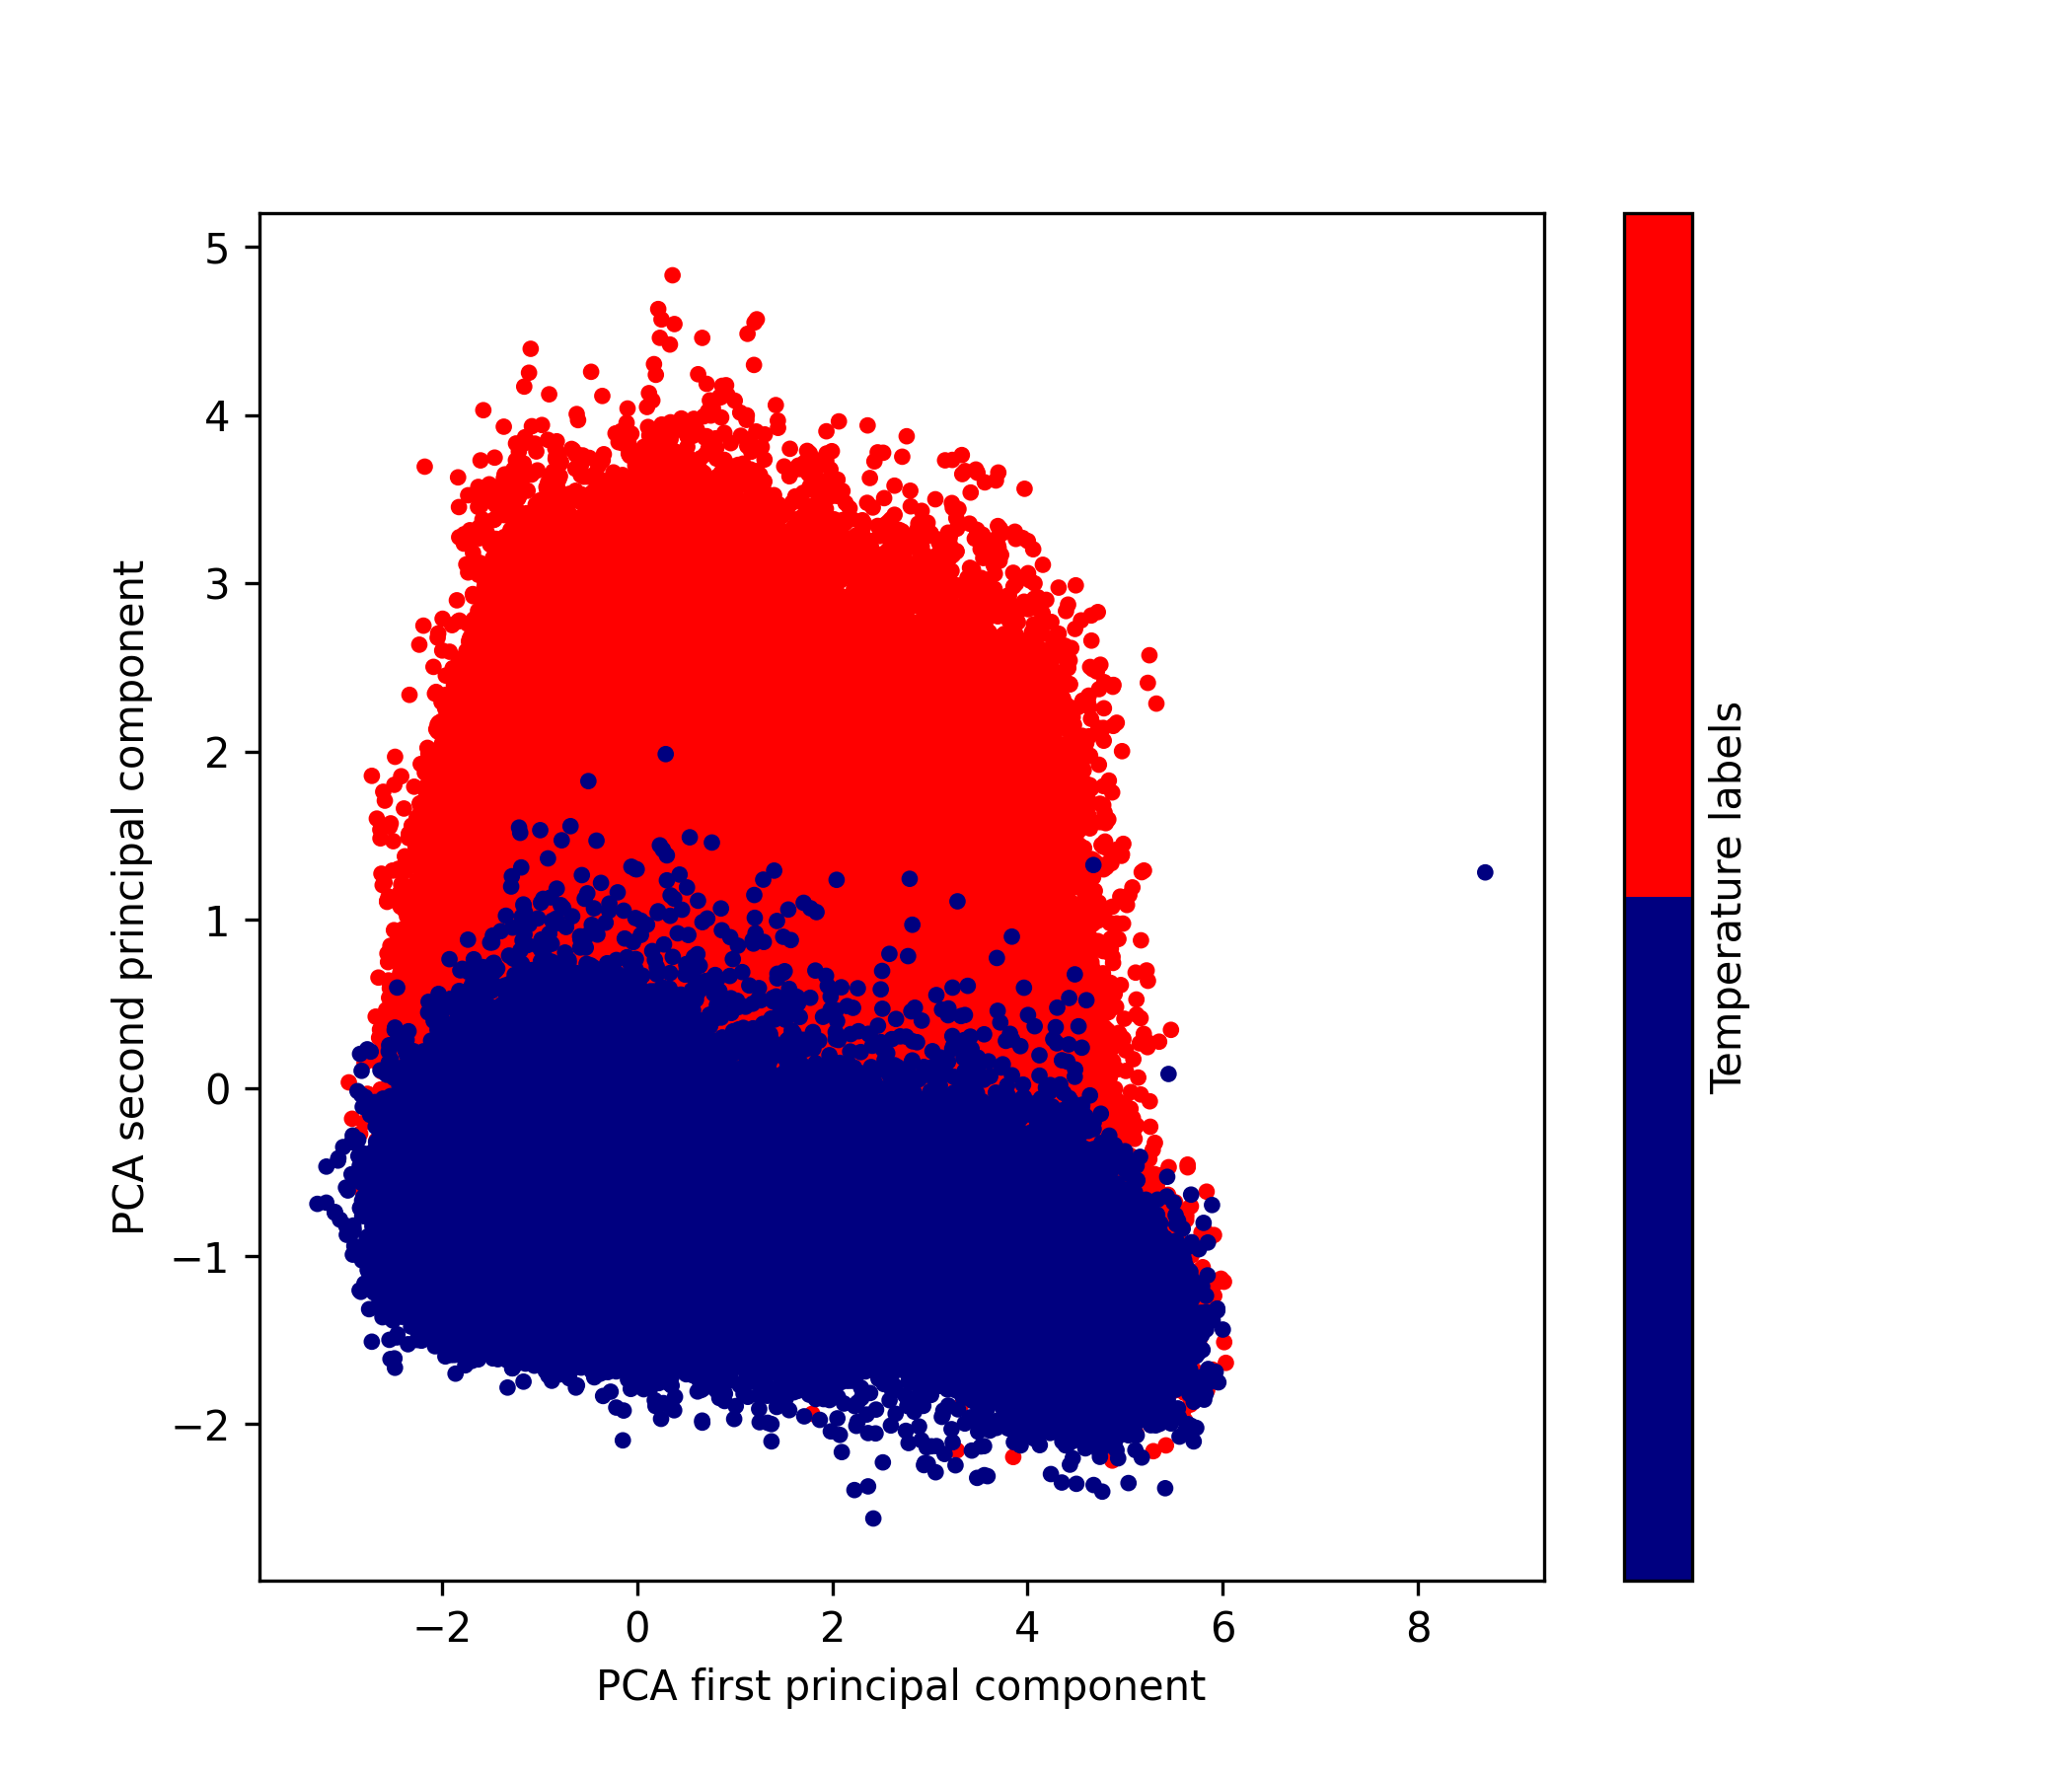
\includegraphics[scale=0.3]{003_train_v2_PCA.png}
		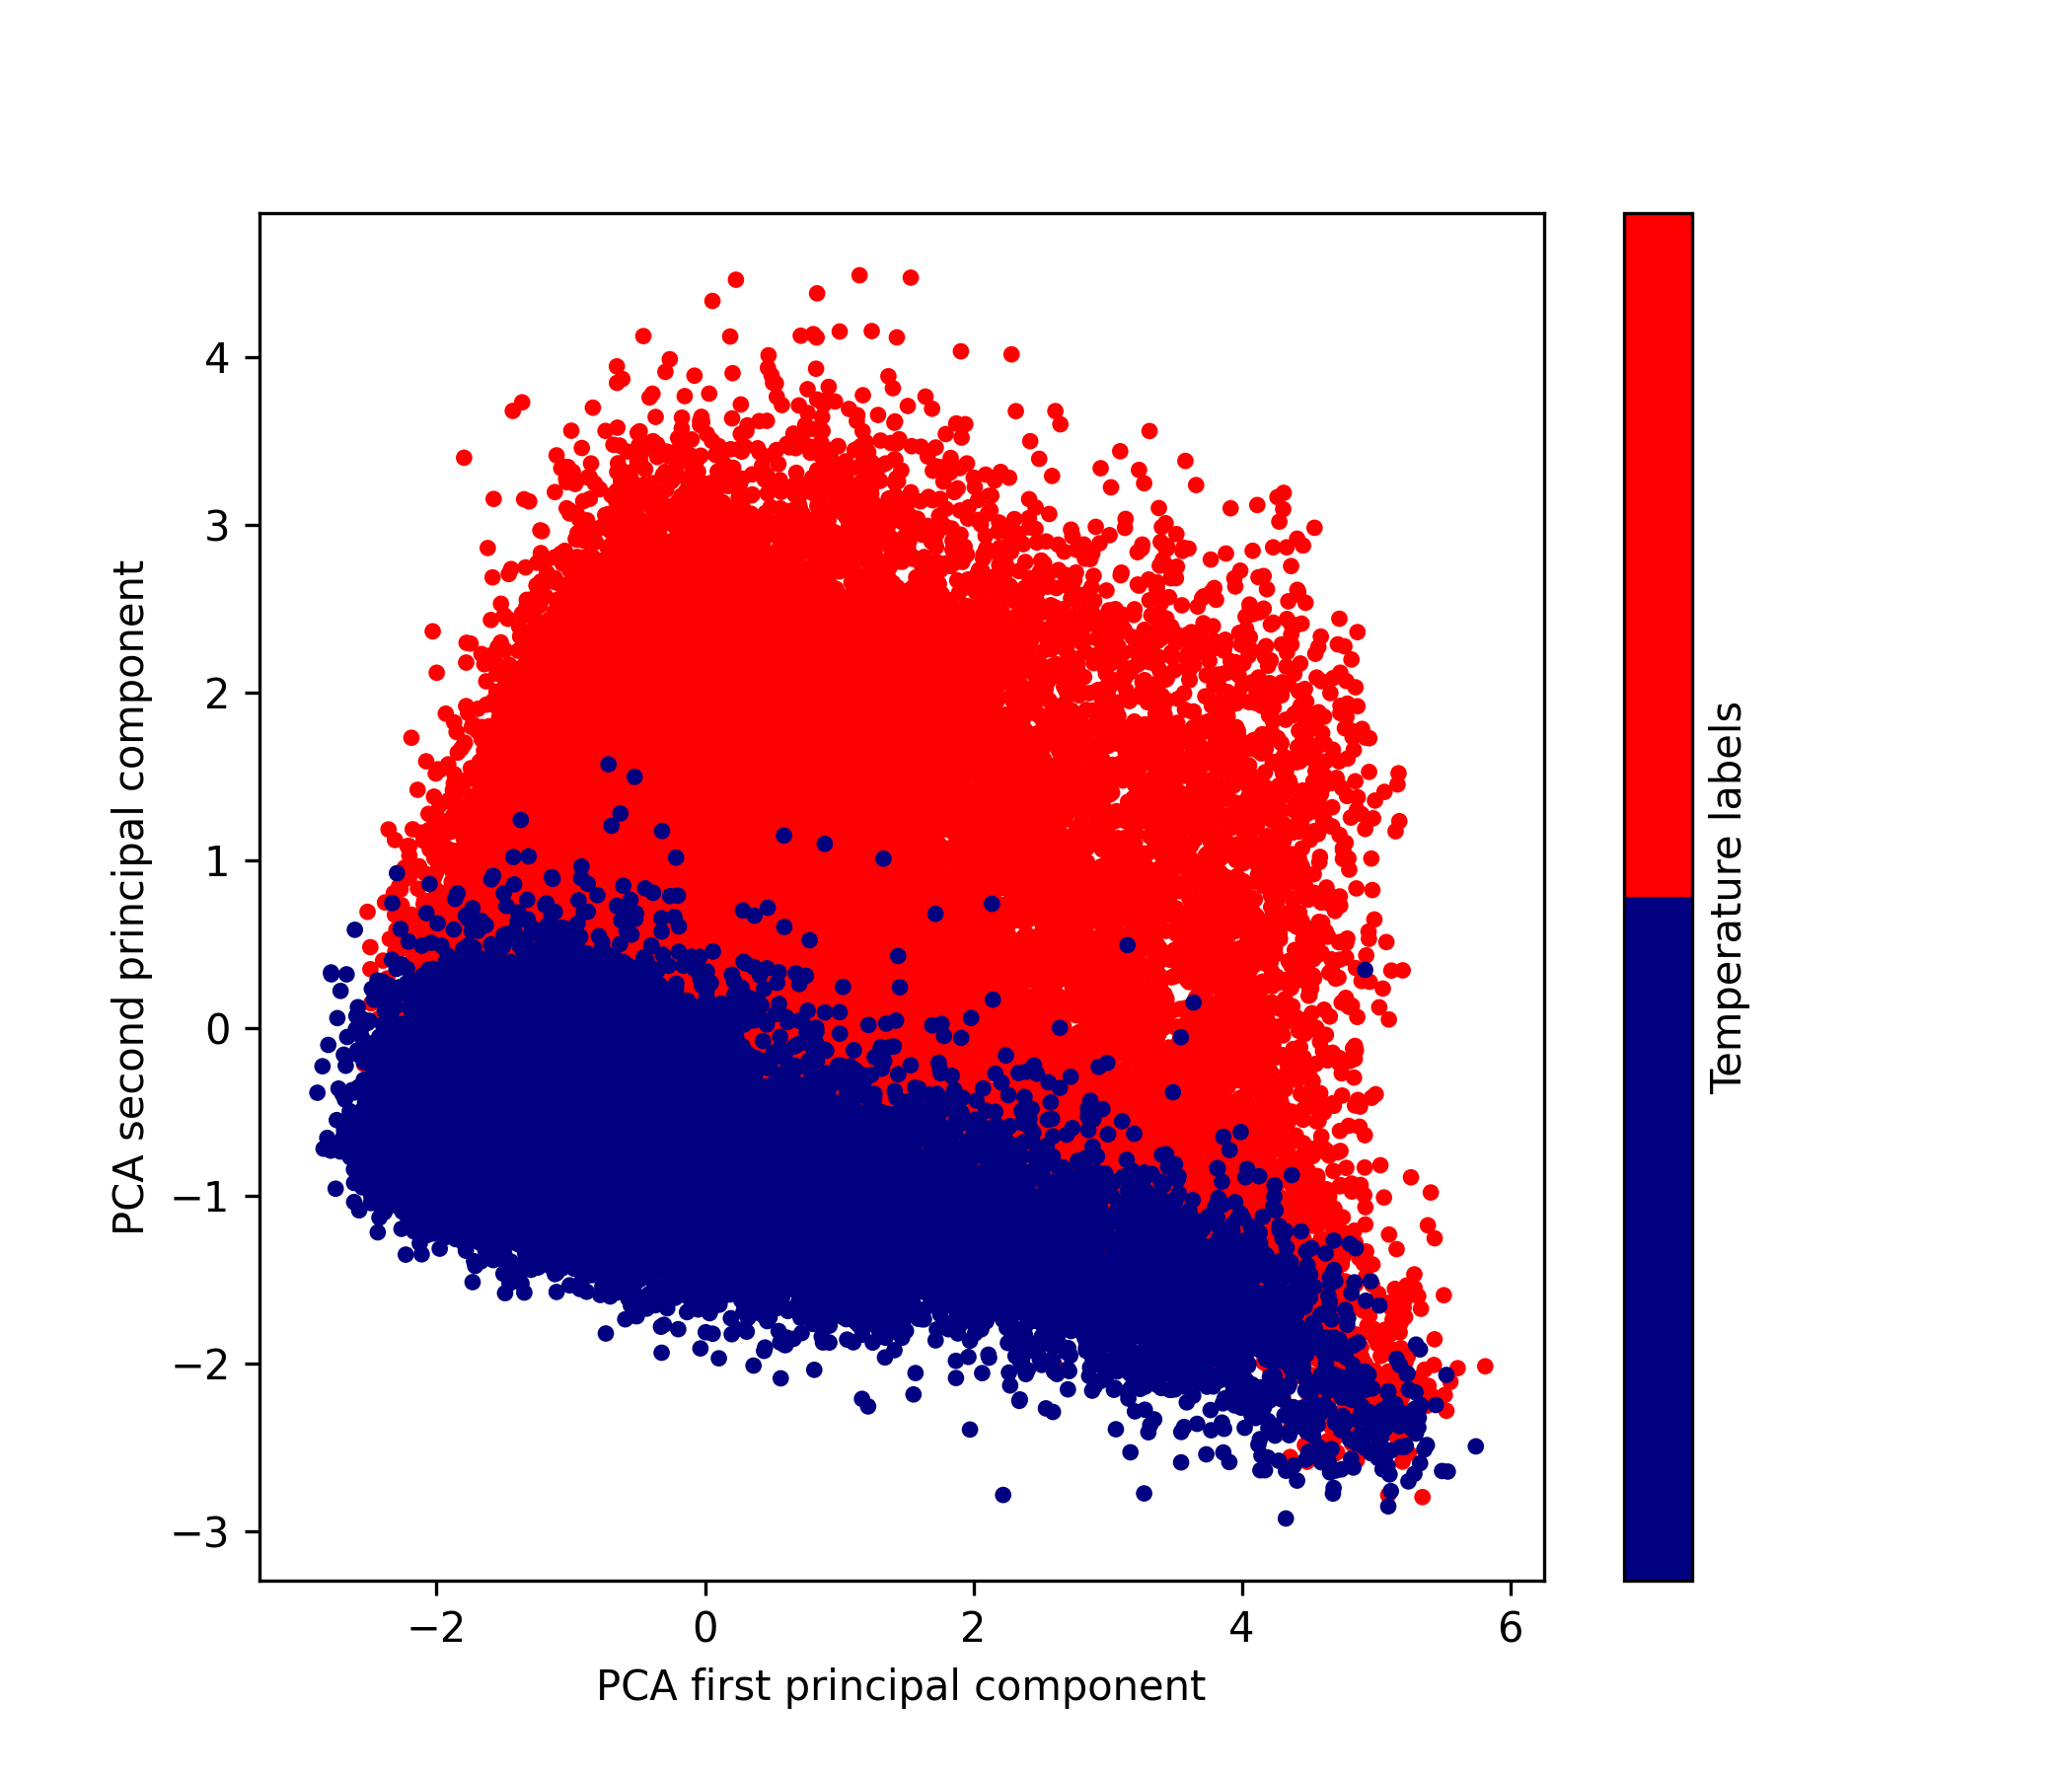
\includegraphics[scale=0.3]{003_validate_v2_PCA.png}

		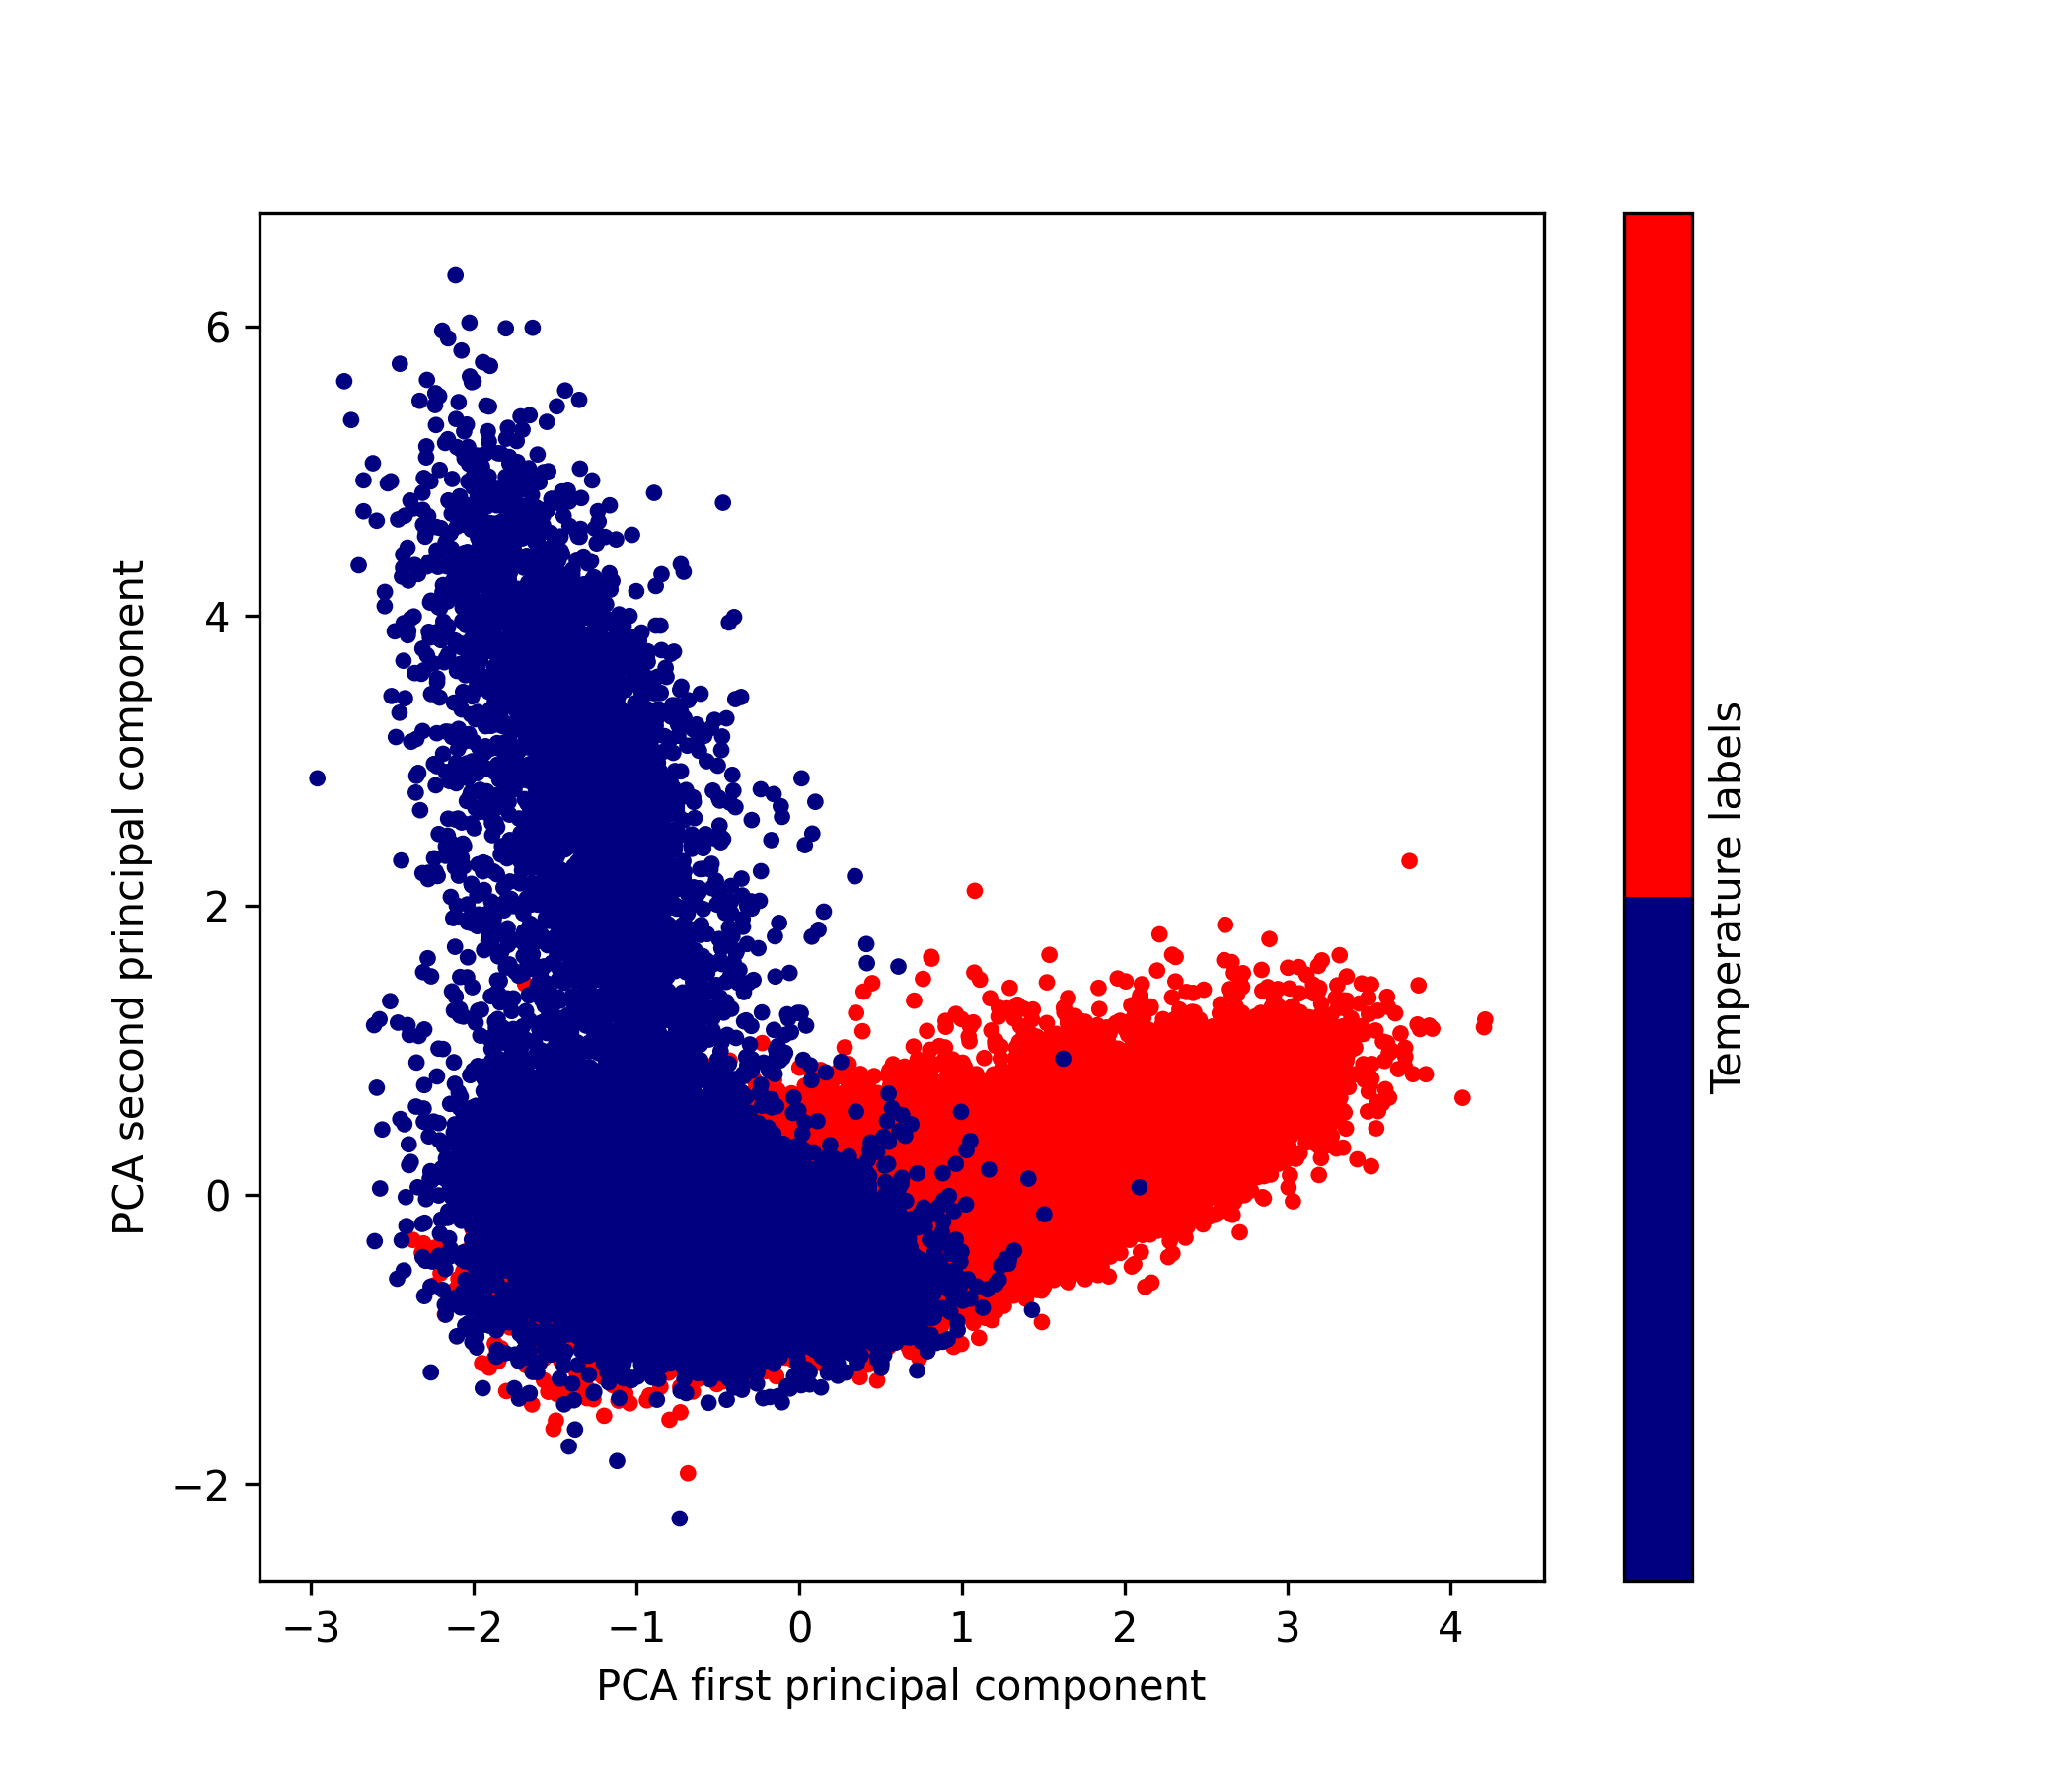
\includegraphics[scale=0.3]{003_test_v2_PCA.png}

		\caption{PCA visualisations of '003' model datasets' embeddings: training set
				in the upper left, validation set in the upper right, and 
				testing set in the lower center}
		\label{figure:ScikitPCAembeddings003}
	\end{figure}
	
	Additionally, \textit{Python} minimum-distortion embedding (\textit{PyMDE}) 
	library (version 0.1.5) was used to visualise datasets of embeddings 
	(Figure \ref{figure:PyMDEPCAembeddings003}).

	\begin{figure}[h!]
		\centering
		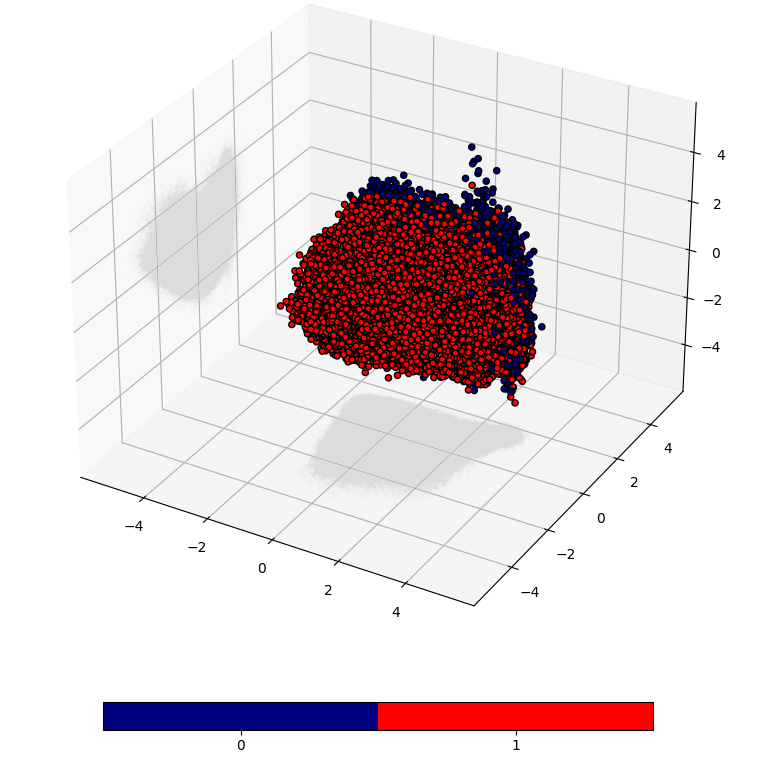
\includegraphics[scale=0.3]{003_train_v2_MDE_PCA.png}
		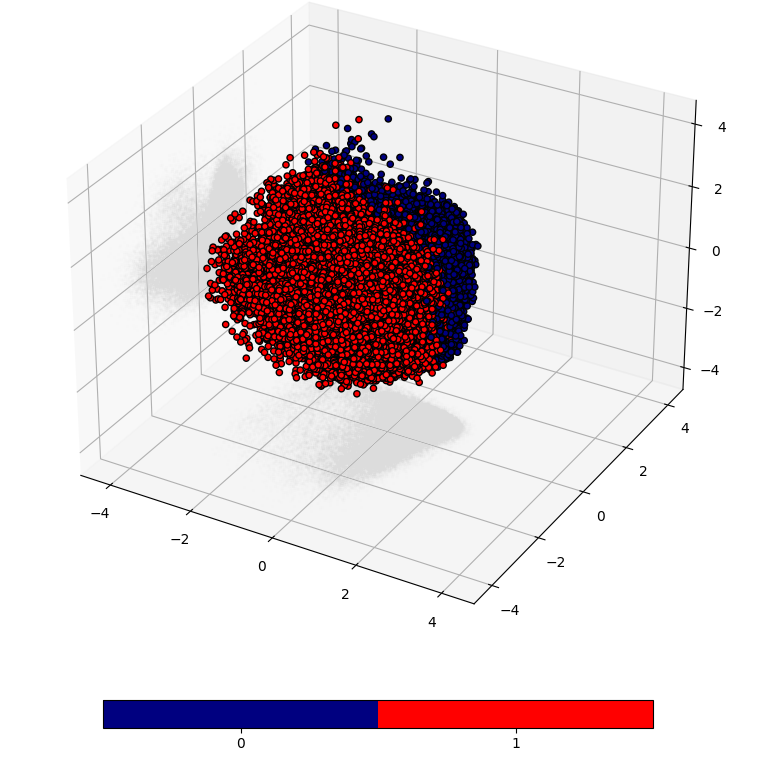
\includegraphics[scale=0.3]{003_validate_v2_MDE_PCA.png}

		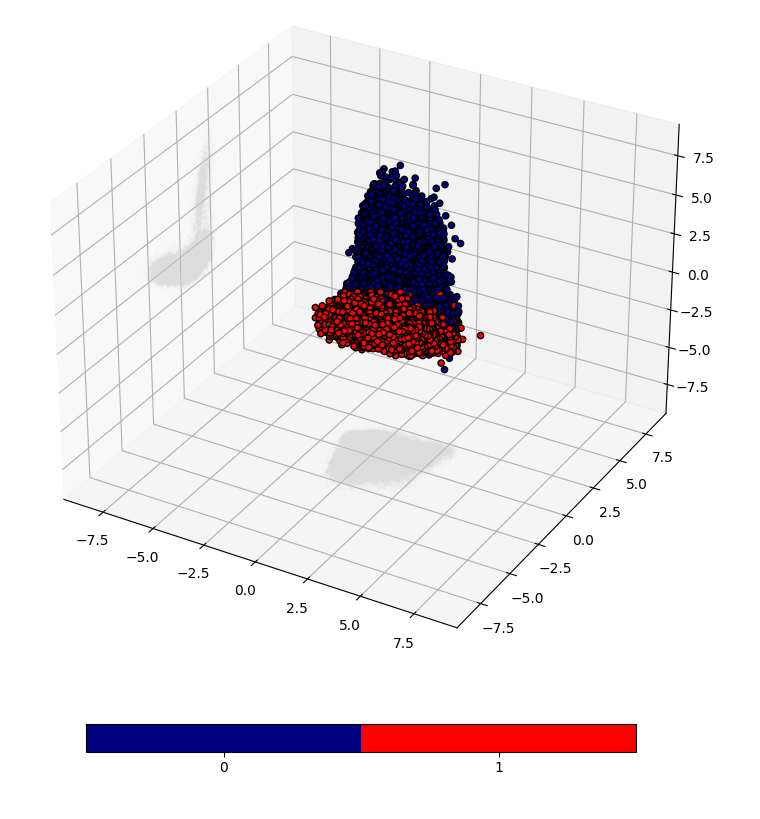
\includegraphics[scale=0.3]{003_test_v2_MDE_PCA.png}

		\caption{\textit{PyMDE} PCA visualisations of '003' model datasets' embeddings: training set
				in the upper left, validation set in the upper right, and 
				testing set in the lower center}
		\label{figure:PyMDEPCAembeddings003}
	\end{figure}

	\newpage

	\subsection{Training and validation of the neural network}

	At first, it was decided to try training the neural network built of
	the most simple architecture - a single layer perceptron (SLP). The input of the 
	layer is 1280-dimensional - it takes the input of protein embeddings - and the 
	output is a binary label that represents the thermostability class. The 
	activation function was chosen to be sigmoid and loss function binary cross
	entropy. Adam optimizer with learning rate of 0.0001 was chosen.

	The model was trained and validated in 5 epochs taking mini-batch size of 24
	embeddings.

	\begin{figure}[h!]
		\centering
		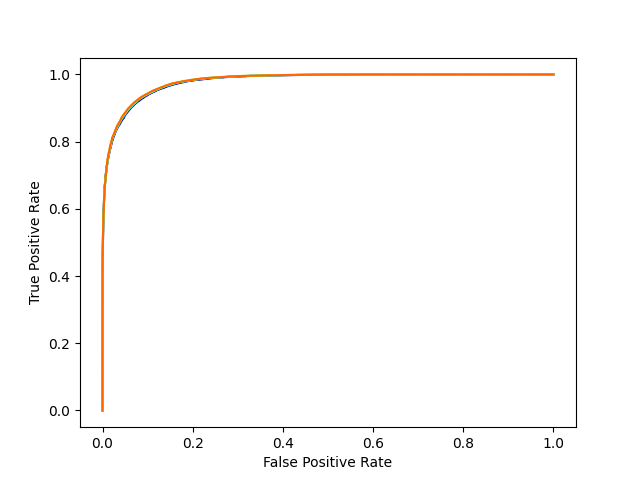
\includegraphics[scale=0.7]{validation_4_2713.png}

		\caption{ ROC curves for each validation epoch - the orange 
		one denotes the curve of the fifth epoch}
		\label{figure:SLP003validation4}
	\end{figure}

	\begin{table}[h!]
		\caption{Confusion matrix after the fifth validation epoch}
		\vspace{0.2cm}
		\centering
		\begin{tabular}{ | c | c | c | }
			\hline 
			& 0 & 1 \\
			\hline  
			0 & 32793 & 3636 \\
			\hline 
			1 & 1582 & 30770 \\
			\hline    
		\end{tabular}
		\label{table:SLP003confusionMatrixValidation4}
	\end{table}

	\begin{table}[h!]
		\caption{Model performance metrics after the fifth validation epoch}
		\vspace{0.2cm}
		\centering
		\begin{tabular}{ | c | c | }
			\hline 
			Accuracy & 0.91989 \\
			\hline  
			Precision & 0.89432 \\
			\hline 
			Recall & 0.9511 \\
			\hline    
			ROC AUC & 0.92 \\
			\hline 
		\end{tabular}
		\label{table:SLP003metricsValidation4}
	\end{table}

	\newpage

	\subsection{Testing of the model}

	The model was tested with the testing subset of '003' dataset that was
	not exposed to the model before the testing stage. 

	\begin{table}[h!]
		\caption{Confusion matrix in the testing phase}
		\vspace{0.2cm}
		\centering
		\begin{tabular}{ | c | c | c | }
			\hline 
			& 0 & 1 \\
			\hline  
			0 & 34933 & 2813 \\
			\hline 
			1 & 2788 & 33122 \\
			\hline    
		\end{tabular}
		\label{table:SLP003confusionMatrixTesting}
	\end{table}

	\begin{table}[h!]
		\caption{Model performance metrics in the testing phase}
		\vspace{0.2cm}
		\centering
		\begin{tabular}{ | c | c | }
			\hline 
			Accuracy & 0.924 \\
			\hline  
			Precision & 0.922 \\
			\hline 
			Recall & 0.922 \\
			\hline    
			ROC AUC & 0.924 \\
			\hline 
			MCC & 0.845 \\
			\hline 
		\end{tabular}
		\label{table:SLP003metricsTesting}
	\end{table}

	\begin{figure}[h!]
		\centering
		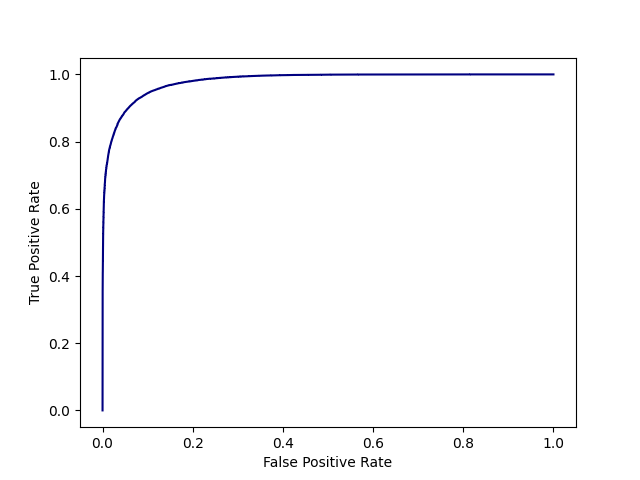
\includegraphics[scale=0.7]{testing_0_3068.png}

		\caption{ ROC curve after the testing stage}
		\label{figure:SLP003testing}
	\end{figure}

	\newpage

	\section{Conclusions}

	\dots

	\nocite{*}
	
	\normalsize

\bibliography{references} 
\bibliographystyle{ieeetr}

\end{document}
